\section{Hardware}\label{Sec_Har}

\subsection{RFID reader and antenna}
The RFID reader from KTS Systeme (see fig.\ref{Reader}) is a HF Modul (frequency around 13.56 MHz). It contains a full-fledged microcontroller with a high-performance RFID transceiver Integrated Circuit (IC). It has a 1.27 mm pitch pin-headers for Through Hole Technology (THT) mounting. The connection to an external antenna can be realized via a single ended 50 $\Omega$ connection or via pin header U.FL. jack, which was used in this project. \\
\begin{figure}[!htbp]
\centering
\includegraphics[width = 8cm]{Pictures/Reader}
\caption{RFID reader KTS Systeme RFIDM1356-001}
\label{Reader}
\end{figure}\\
The communication to other devices is realized via a Universal Asynchronous Receiver-Transmitter (UART) compatible serial interface via pin 6 (RX) and 7 (TX). The power supply is a 5 V DC connection via pin 1 (VCC) and pin 10 (GND). The reader is standardized to ISO 15693 and ISO14443A/B and has the overall dimensions 36 x 16 x 4 mm [LxWxH]\cite{KTSSysteme.2017}.\\
The reader has three LEDs:
\begin{itemize}
	\item Green: Run - Lights when reader receives power
	\item Yellow: Tag - Lights when a tag is detected
	\item Red: Data - Lights when data transfer to or from a tag
\end{itemize}
To configure the reader, KTS Systeme also provides a software (Tag2Image) for free. The reader was configured to scan the environment in an automatic anti collision mode (AT+Scan=AC,RSSI). Anti collision means that multiple tags can be detected at the same time and is highly important in this project. The output of the scan is a continuous information of the Identification (ID) and the Received Signal Strength Indicator (RSSI) of the detected tags. For example: SCAN:+UID=E00402000018313E,+RSSI=7/6 means that the tag with the ID (in hex) E00402000018313E was detected with a RSSI of 7/6. For the RSSI is the first number the value for the main and the second for the auxiliary receiver channel. In this project only the first number of the RSSI was used, because they are almost the same. The RSSI is an integer value from 0 to 7 and gives an information about the distance between the antenna and the detected tag. 0 stands for the maximum reading range which was mentioned to be around 15 cm. A detailed relation was obtained through experiments during the project and will be explained later in this report. An AT Command Reference Guide is also available on http://rfid.kts-systeme.de/downloads/.\\
\\
The antenna (fig. \ref{Antenna}) is a HF PCB Antenne (PCBA1356$\_$8) also from the company KTS Systeme. It has a dimension of 80 x 80 mm. The connection to the reader is realized by a SMA jack and has a self-impedance of 50$\Omega$. The antenna is designed for passive tags in a frequency range around 13.56 MHz and has a maximum power of 1W. \\
\begin{figure}[!htbp]
\centering
\includegraphics[width = 6cm]{Pictures/Antenna}
\caption{RFID Antenna KTS Systeme PCBA1356$\_$8}
\label{Antenna}
\end{figure}\\
The antenna and the reader are connected with a SMA to U.FL. adapter cable.\\

\subsection{RFID tag}
The tag used in the prototype is of paper type (see fig.\ref{tag}) due to its added advantages as follows:
\begin{itemize}
	\item The tags are cheap costing 18 cents each.
	\item It doesn't require power supply.
	\item The tags are compact.
	\item The implementation in the time of plant extension is simple.
\end{itemize}
\begin{figure}[!htbp]
	\centering
	\begin{minipage}{.5\textwidth}
		\centering
		\includegraphics[width = 6cm]{Pictures/tag}%
		\caption[The ListOfFigures caption]{Paper Tag \footnotemark[1]}
		\label{tag}
	\end{minipage}%
	\begin{minipage}{.5\textwidth}
		\centering
		\includegraphics[width = 6cm]{Pictures/tagsfloor}%
		\caption{Tags on the plant floor}
		\label{tags_floor}
	\end{minipage}
\end{figure}
It's working principle is based on inductive coupling with an operating frequency of 125-135 kHz and a range of 10cm. The tags are fixed on the floor at known location as shown in fig.\ref{tags_floor}.
\subsection{Wifi Module}
The WiFi module used is from WEMOS Co.\cite{wemosd1mini}.It is a mini WiFi board with 4MB flash based on ESP-8266 which is a WiFi microchip with full IP/TCP stack and micro-controller (see fig.\ref{wemos}).
\footnotetext[1]{Source: \url {www.kurzweilai.net/scientists-print-cheap-rfid-tags-on-paper}}
\footnotetext[2]{Source:\url{ www.github.com/mcauser/Fritzing-Part-WeMos-D1-Mini}}
\begin{figure}[!htbp]
	\centering
	\includegraphics[width = 5cm]{Pictures/wemos}
	\caption[The ListOfFigures caption]{WeMos D1 Mini WiFi Module \footnotemark[2]}
	\label{wemos}
\end{figure}
\\
The WeMos module has the following features:
\begin{itemize}
	\item 32-bit RISC microprocessor core running at 80 MHz
	\item External QSPI flash of 4 MB
	\item IEEE 802.11 b/g/n Wi-Fi
	\item 16 GPIO pins
	\item UART on dedicated pins, plus a transmit-only UART can be enabled on GPIO2
	\item 10-bit ADC and \(I^2C\) (software implementation)
\end{itemize}
\subsection{Hardware Setup}
\begin{figure}[!htb]
	\centering
	\includegraphics[width = 13cm]{Pictures/roboschematic}
	\caption{Robot Hardware Schematic}
	\label{robo_schematic}
\end{figure}
The built-in Micro-controller on the robot receives the sensor data and sends commands to the actuators via serial communication using its first UART pins. (TX/RX) is the process of sending and propagating an analogue or digital information signal over a physical point-to-point wired connection. It uses its second UART pins to communicate with the built-in WiFi Module. The built-in WiFi Module sends the received sensors data to the Computer and sends the received commands from the computer to the robot micro-controller via Wireless communication (see fig.\ref{robo_schematic}).
\begin{figure}[!htb]
	\centering
	\includegraphics[width = 11cm]{Pictures/hwschematic}
	\caption{Hardware Schematic}
	\label{hw_schematic}
\end{figure}
Due to its less complexity, more flexibility and that the robot's in built micro-controller UART pins are in use, a new communication setup was developed for the RFID reader to send the data from the robot to the computer in parallel to the robot hardware setup. As shown in fig.\ref{hw_schematic}) the RFID reader is connected directly to the built-in micro-controller of the WeMos WiFi Module via serial communication sending it the tags IDs. The WeMos WiFi Module sends the received data through the network. The RFID reader is connected to the antenna which sends and receives the radio waves via SMA antenna cable.\\
The RFID reader as well as WeMos Module are placed on the top of the robot while the Antenna is fixed to the robot base such that the radio waves would be in direct contact with the tags on the floor.
\begin{figure}[!htbp]
	\centering
	\begin{minipage}{.5\textwidth}
		\centering
		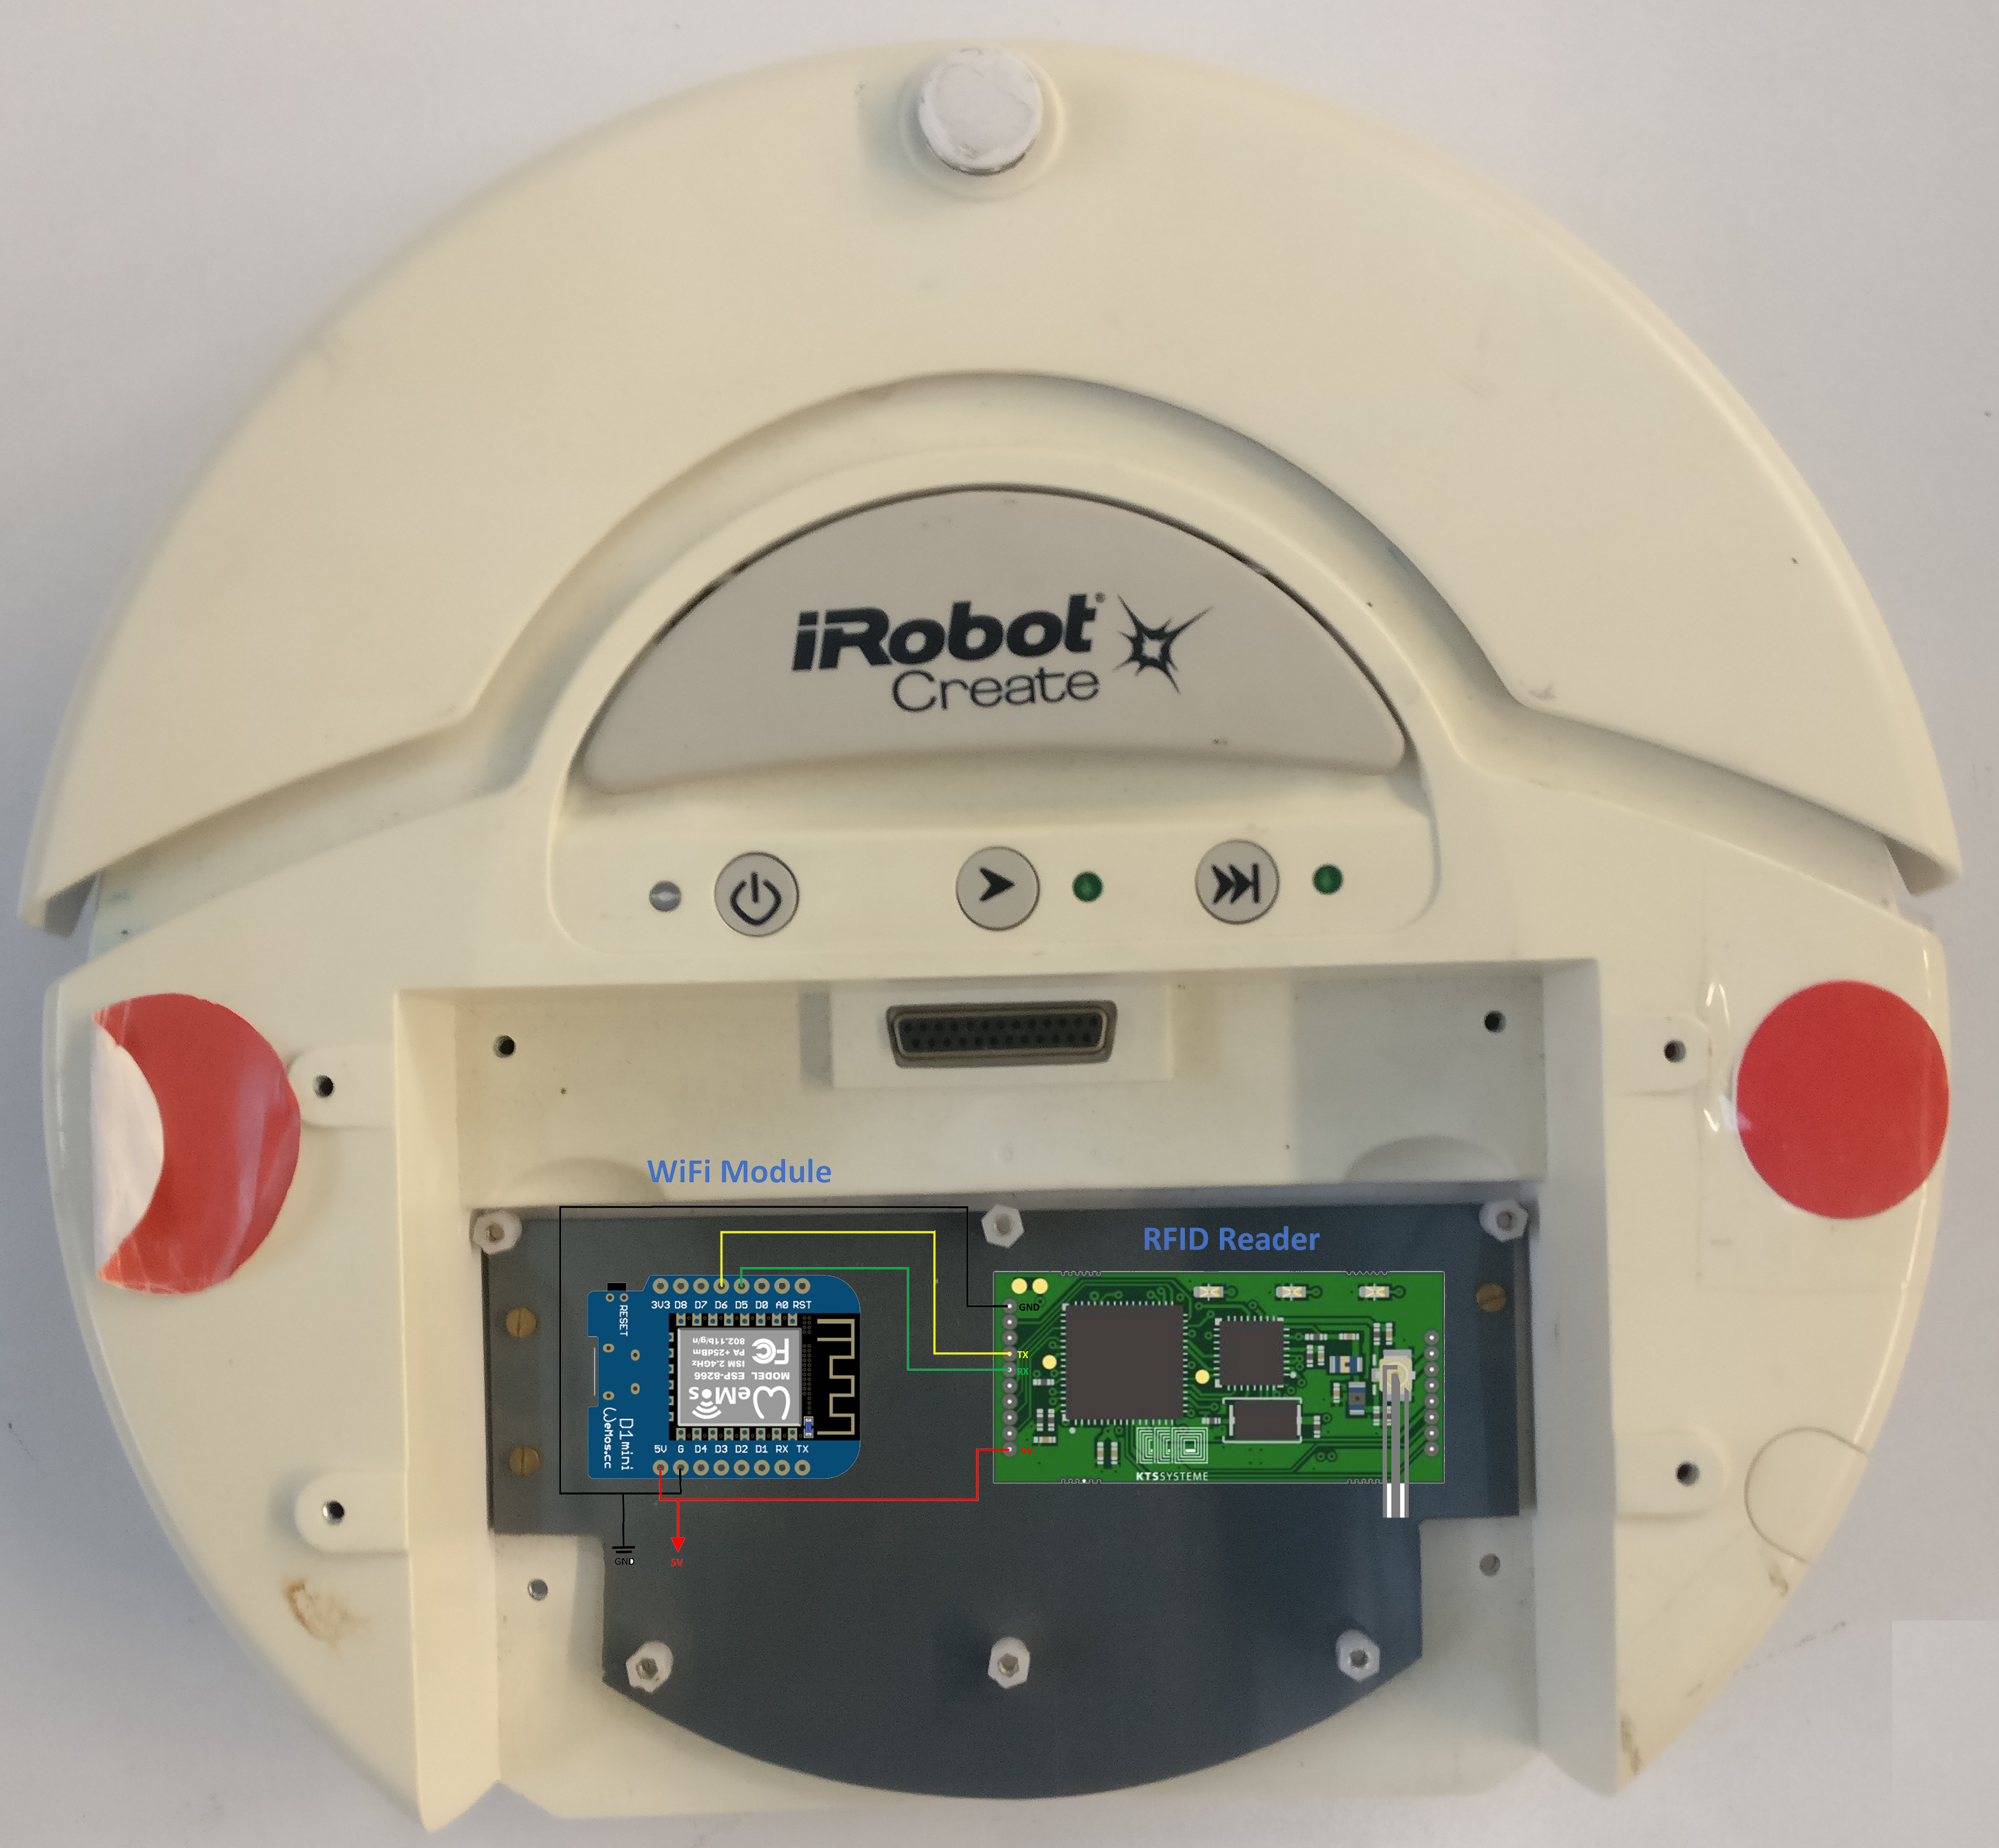
\includegraphics[width = 5cm]{Pictures/rfidonrobot}%
		\caption{Top of the Robot}
		\label{rfid_on_robot}
	\end{minipage}%
	\begin{minipage}{.5\textwidth}
		\centering
		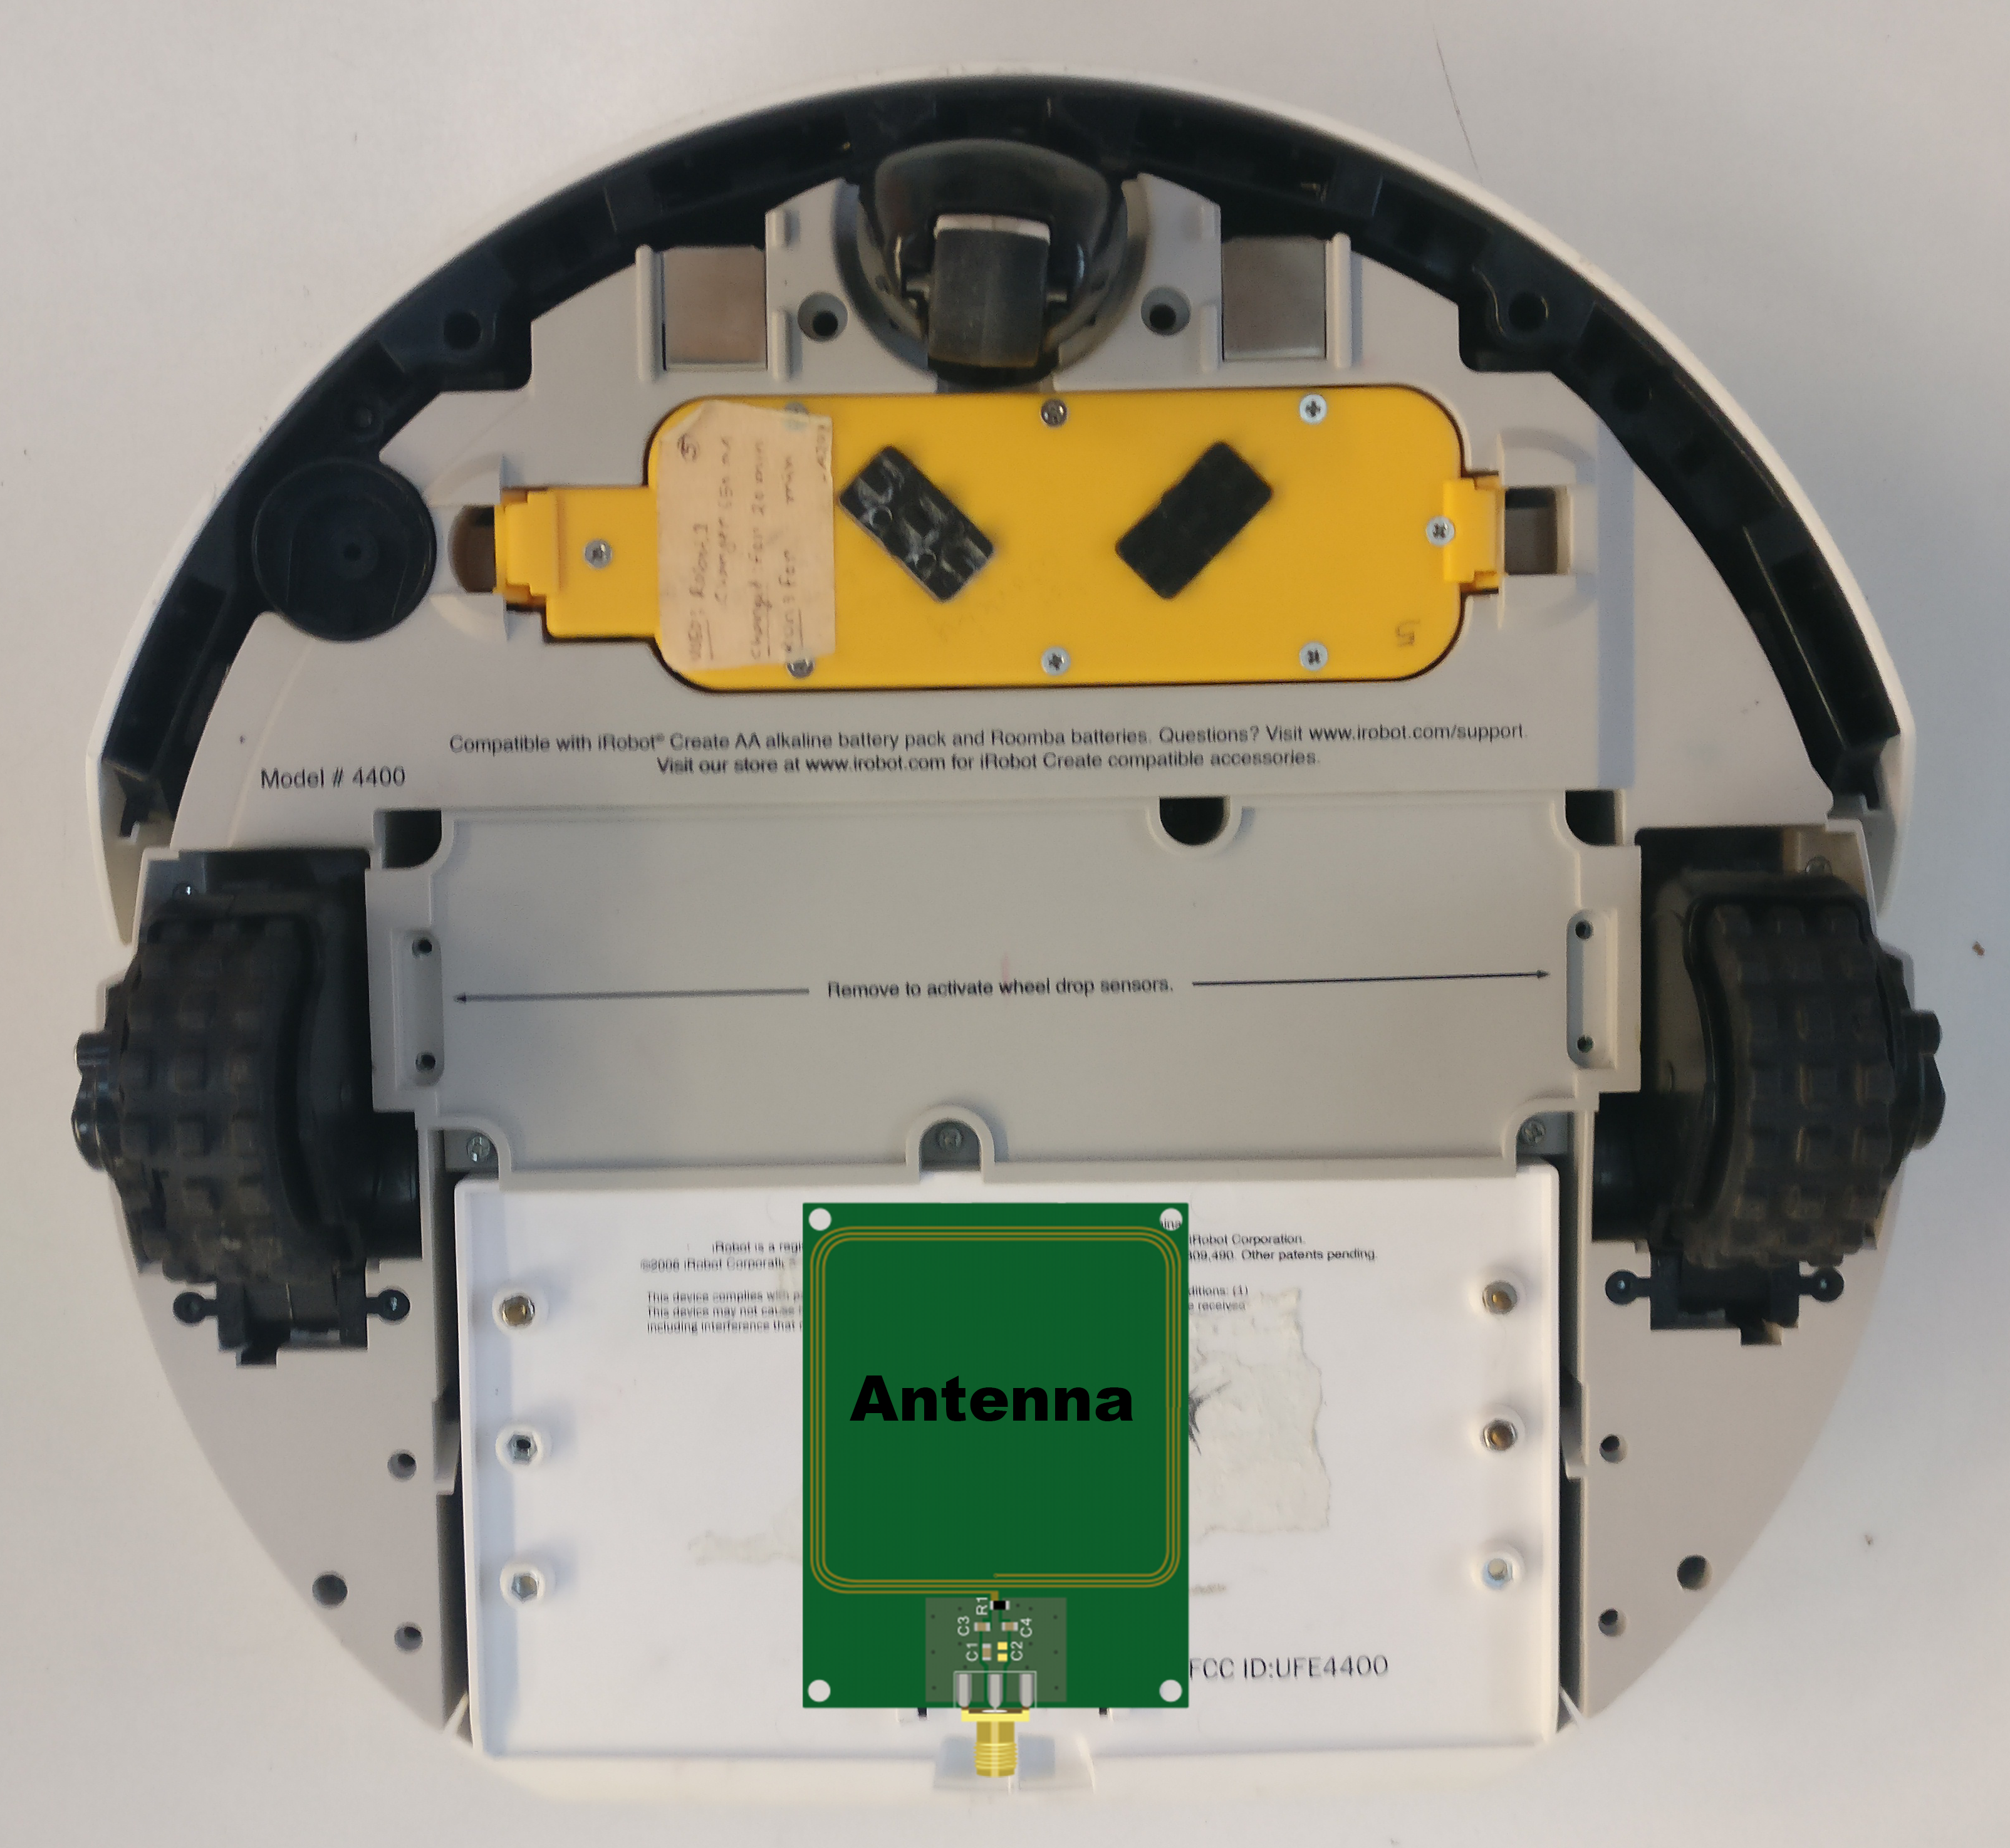
\includegraphics[width = 5cm]{Pictures/antennaonrobot}%
		\caption{Base of the Robot}
		\label{antenna_on_robot}
	\end{minipage}
\end{figure}